\documentclass{article}
\usepackage{enumitem}
\usepackage{amsmath}
\usepackage{tikz}
\usepackage{graphicx}
\linespread{1.5}
\usepackage[a4paper,
            bindingoffset=0.2in,
            left=0.8cm,
            right=0.8cm,
            top=0.8cm,
            bottom=0.8cm,
            footskip=.25in]{geometry}
\usepackage{fancyhdr}
\usepackage[style=authoryear]{biblatex}
\addbibresource{refs.bib}
\begin{document}
\pagestyle{fancy}
\fancyhf{} % clear existing header/footer entries
\fancyfoot[R]{\fontsize{8}{12}\selectfont \thepage \hspace{0.02cm}}
\fancyfoot[C]{\fontsize{8}{12}\selectfont 1163165}
\fancyfoot[L]{\fontsize{8}{12}\selectfont Javed Alam}


\begin{center}
  \Large\textbf{Privacy and Security in the Digital Age}\\
  \small{The emergent ethical and security concerns arising from publicly available facial recongition technology}
\end{center}
\section*{\fontsize{10}{12}\selectfont Introduction}

The first quarter of the twenty-first century has been characterised by rapid advancement development and innovation. The maturation of deep-learning algorithms has brought into reality concepts that previously existed only in the imagination. However, with great power comes great responsibility. As powerful new technologies are developed, and existing technologies are refined, novel privacy and security concerns arise. Since the advent of social media, with the creation of MySpace in 2003, a growing number of individuals have uploaded both photographs of themselves, and sensitive personal information to the internet. Much of this personal information would have been uploaded by users of an age unable to fully comprehend the consequences of doing so. Unfortunately, the statement that "nothing gets deleted on the internet" has proven to be remarkably accurate.
\vspace{0.3cm} \\ 
Internet scrapers are automated algorithms that crawl the internet and save data to local storage. Almost half of internet traffic now comprises scraping bots (\cite{conde2024five}). Scrapers do serve legitimate purposes; search engines, for example, require scrapers to discover and index as many websites online as possible. These scrapers discover new websites by going from link to link and recording the metadata associated with each page. Similarly, archiving services such as the Internet Archive use scrapers to save a 'copy' of pages on the internet at different time-points for historical purposes. However, scrapers can also be used for more nefarious purposes. Personal data has value, and the internet contains a lot of it. Data brokers and other businesses are now scraping the internet specifically for personal or identifying information that can be sold to third parties or the public.
\vspace{0.3cm} \\
This information is sold by websites known as "People Searching Websites" (PSWs). PSWs essentially create profiles containing personal information without the subject's consent. These profiles are searchable by name, and contain home addresses, phone numbers and e-mails. Disturbingly, some PSWs also have sensitive details such as the make and registration of family vehicles, estimated income, and names of relatives (\cite{take2024expect}).
\vspace{0.3cm} \\
A novel and highly consequential form of data scraping is the scraping of biometric data. The two types of biometric data available online are voice recordings and images of faces. The percentage of Australian adults with a recording of their voice online is 43\%, while 86\% of US adults have at least one photograph of themselves online (\cite{CyberSecurity2023}, \cite{YouGov2022}) . The primary risk associated with scraping of voice recordings is voice-cloning scams, where artificial intelligence is used to clone the voice of an individual, and ask for money from a relative or friend. However, the indiscriminate scraping of facial biometric data (FBD) poses a unique threat to privacy.
\vspace{0.3cm} \\
\textit{ClearView} and \textit{PimEyes} are two companies that offer facial recognition technology 'search engines'. \textit{ClearView} is only available to government services and private business, but has expressed interest in providing its services publicly. PimEyes is publicly available, and costs \$51.99 AUD per month for up to 25 searches per day on their cheapest plan. The most expensive plan costs \$518.99 per month and allows for a more thorough searching feature (\cite{PimEyes2024}). Both \textit{ClearView} and \textit{PimEyes} have developed sizeable facial-recognition databases through the large-scale indiscriminate scraping of FBD from numerous different internet sources, including social media, news sites, video hosting websites (such as YouTube), forums and pornographic websites.
\vspace{0.3cm} \\
The images are analysed with deep-learning facial recognition algorithms to create a 'faceprint' of each individual. These algorithms measure features such as the spacing of the eyes, width and height of the nose, depth of the eye sockets, shape of the eyes, and shape of the mouth, to create a unique numerical code that corresponds to an individual's face. They then associate each faceprint with all the images containing that face. When a user performs a 'search' by uploading a picture of a person, the algorithm will generate a faceprint for the pictured individual, and match it to the most similar faceprint within the system's database. The website will then return all photographs that the pictured individual has posted online, in addition to the webpages from which they were obtained, and potentially sensitive personal data on those websites (e.g., the associated text from a social media post accompanying the original photograph.)


\section*{\fontsize{10}{12}\selectfont The Challenges to Privacy, Security and Ethics}
The combination of publicly available facial recognition technology and PSWs allows any individual with a camera and internet connection to identify and find personal information about any individual that they come into contact with (\cite{conde2024five}). The power of combining these technologies was recently demonstrated by two students from Harvard University who developed an application called 'I-XRAY' for demonstrative purposes. The application automates the process of uploading a face from a live image provided by smart glasses or mobile phone, and returning detailed information about the pictured individual, such as their name, address, phone number, e-mail, occupation, and selected life events. The application uses a deep-learning image-detection algorithm to locate and screencapture a face within the live image, and automatically perform a search on PimEyes. In addition to other photographs of the individual, PimEyes also returns all URLs on which the individual's photographs were hosted. These URLs usually contain identifying information, for example, the name on a social media profile. A service called FireCrawl is then used to scrape these URLs and obtain identifying information. This identifying information is then used to perform an automated search on a PSW, thereby returning the individual's name, address, phone number, e-mail, and sensitive personal details. Finally, a Large Language Model (LLM) is then used to compile the photographs and personal information of the pictured individual into a profile for viewing on an electronic device.
\vspace{0.3cm} \\
While this application has not been publicly released, the steps involved can be achieved by any person with a basic level of technological literacy. Clearly, these technologies pose significant ethical, privacy and security concerns. The scraping of individuals' personal FBD without their consent and development of the associated faceprint constitutes a violation of the human right to privacy.
\vspace{0.3cm} \\
There are multiple ways in which these technologies can be used in a criminal manner. An assailant no longer has the need to follow a potential victim home; a photograph will now be sufficient to obtain the victim's address. While there have yet to be any recorded physical crimes committed with the assistance of this technology, it seems inevitable that there will be in the future. A disturbing example of the potential criminal applications is the harassment of pornographic actors. PimEyes has been used by malicious individuals to locate the social media profiles and addresses of pornographic actresses, for the purpose of exposing them to their friends and families (\cite{Kiene2024}). The Russian equivalent, 'FindFace', has also been used in a similar manner, and in Germany, one individual created a databse of pornographic actresses social media profiles, to allow males to screen their female partners (\cite{SophosNews2019}).
\vspace{0.3cm} \\
While facial-identification technology represents a significant threat to privacy and personal security, other uses of facial analysis pose unique challenges. In addition to indicating gender, age, and ethnicity with a reasonable degree of accuracy, the expressions on a face provide highly dynamic data about an individual's emotions and state of mind (\cite{conde2024five}). Many businesses now employ facial recognition technology within their stores, with implied consent provided by customers on the basis of witnessing a sign within the storefront (\cite{Vladimirova2024}). The claimed purpose is to prevent theft, however, there is nothing precluding such businesses from analysing customers' facial expressions in response to viewing specific items within the store for the purposes of market research.
\begin{center}
{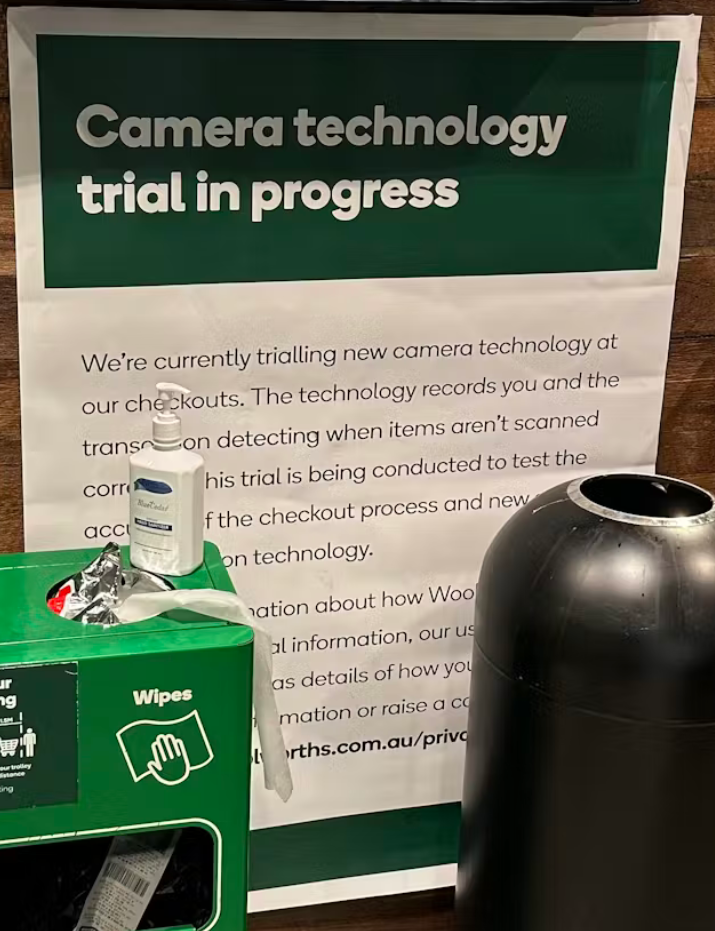
\includegraphics[width=0.5\textwidth]{signcropped.png}}
\end{center}
Of particular concern are algorithms that can predict biological, neurological, and psychosocial traits from the face of an individual (\cite{conde2024five}). For example, \cite{Wang2018} developed a deep-learning algorithm that could determine whether a pictured male was homosexual or heterosexual with 81\% accuracy. Conversely, humans who performed the same task were only able to achieve 61\% accuracy. Homosexual women were detectable with 71\% accuracy by the algorithm, compared to 57\% accuracy for human evaluators. Sexual orientation is highly personal and private information, which now may be detectable upon entrance into any store.        
\vspace{0.3cm} \\
In another concerning example, a facial recognition algorithm correctly classified political orientation in 72\% of 1,085,795 images of liberal and conservative face-pairs, a rate significantly higher than random chance. This accuracy was also higher than human evaluators (55\%) and a 100-question personality survey (61\%) (\cite{Kosinski2021}). These two examples, while alarming, are not outliers in the field of facial analysis. There exist many different types of algorithms that are able to use the power of large datasets and deep learning to make predictions about almost any aspect of an individual from their face. Within a late-stage capitalistic society, it is inevitable that businesses will take advantage of such algorithms to increase their profits if they are not prevented by the law.
\vspace{0.3cm} \\
In summary, publicly available facial recognition technology and people searching websites pose risks to physical security and constitute an invasion of privacy. Additionally, novel uses of facial analysis are proving highly accurate in the detection of many different biological and psychosocial features, and pose what is likely the greatest threat to privacy within this century.
\section*{\fontsize{10}{12}\selectfont Current Solutions}
Australian Privacy Act, ClearView Legal Challenge
% \printbibliography
\end{document}